%!TEX root = ../document.tex
\chapter{Scientific background}
In this chapter we will first give some basic intro to photosynthesis, then proceed to some monitoring and automated systems, which will lead to the next chapter, an introduction to Monoplant and its technical specifications.

\section{Photosynthesis}
The variables that we monitor in our application are directly linked to the precondition of all life, photosynthesis. During this process plants transform energy from light to chemical energy in the form e.g glucose and starch. As most organisms are not able to make use of light energy directly, plants are a necessity for producing energy that other organisms can transform. In addition, oxygen is generated as a waste product of the process, enabling us to breathe. The equation for photosynthesis is written as: \ce{(CO2)n + (H2O)n + photons -> (CH2O)n + (O2)n}, which means that carbon dioxide, water and light transforms to glucose and oxygen.  

Photosynthesis consists of two main parts: the light-dependent reactions, and the light-independent reactions. The light-dependent reaction, as the name implies, occur only in the light. The light-independent reaction occurs both in the light and dark, but does not rely on solar energy.  

\begin{figure}
\centering
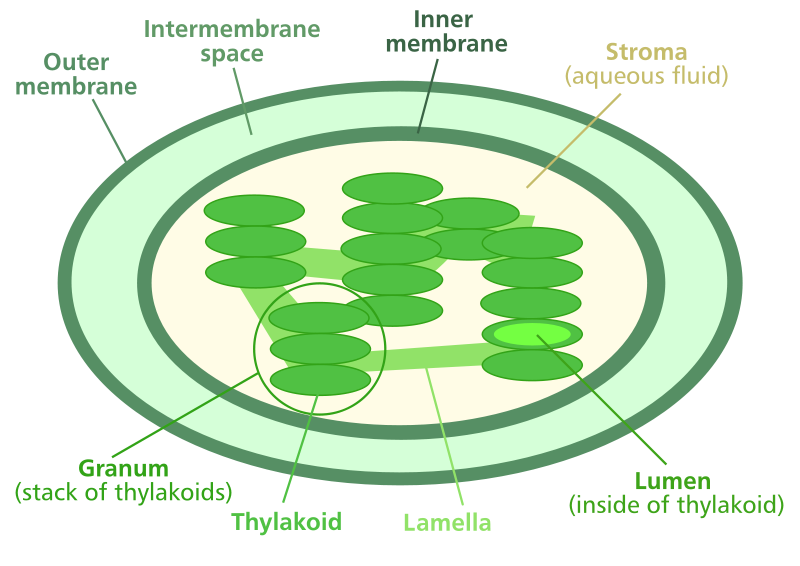
\includegraphics[width=0.8\textwidth]{img/photosynthesis/Chloroplast_diagram.png}
\caption{Illustration of a chloroplast molecule \citep{wiki:chloroplast}}
\label{fig:chloroplast}
\end{figure}

\subsection{Light-dependent reaction}
The light-dependent reaction consists of two different photosystems (photosystem 1 and photosystem 2) creating adenosine triphosphate (ATP) and nicotinamide adenine dinucleotide phosphate (NADPH) molecules for the light-independent reactions. Both systems are located in the thylakoid membrane inside the chloroplast organelles (see figure~\ref{fig:chloroplast} on page~\pageref{fig:chloroplast}). In the process, photosystem 2 precedes photosystem 1 as photosystem 1 was discovered first. 

\subsubsection{Photosystem 2}
In photosystem 2, antenna-complexes consisting of pigments, proteins and enzymes absorb light of different wavelengths and transfer the energy to chlorophyll molecules \citep{bios}. The energy leads to electrons jumping to an orbit lying further from the nucleus, making the atom excited. This makes the atom unstable, and a perfect candidate for giving away its electrons to electron-acceptors in an electron-transport chain.

Since the chlorophyll loses two of its electrons in the process, it gets positively charged and need to find new electrons somehow to be able to absorb photons again. This happens by taking two electrons from a water molecule absorbed by the plant's roots, which then gets split into \ce{2H+} and \ce{1/2O2} \citep{bios}. The oxygen dissolves in the air, while the hydrogen protons are “trapped” on the inside of the thylakoid membrane (lumen). This makes the lumen positively charged relative to the stroma, which enables generation of ATP-molecules from ADP- and P-molecules. 

\subsubsection{Photosystem 1}
Photosystem 1 consists of the same parts as photosystem 2, but instead of splitting water molecules, it receives two electrons from the electron transport chain in photosystem 2. These electrons gets transferred out in the stroma, and are then tied together with an h+-proton and NADP+ to produce NADPH.

\begin{figure}
\centering
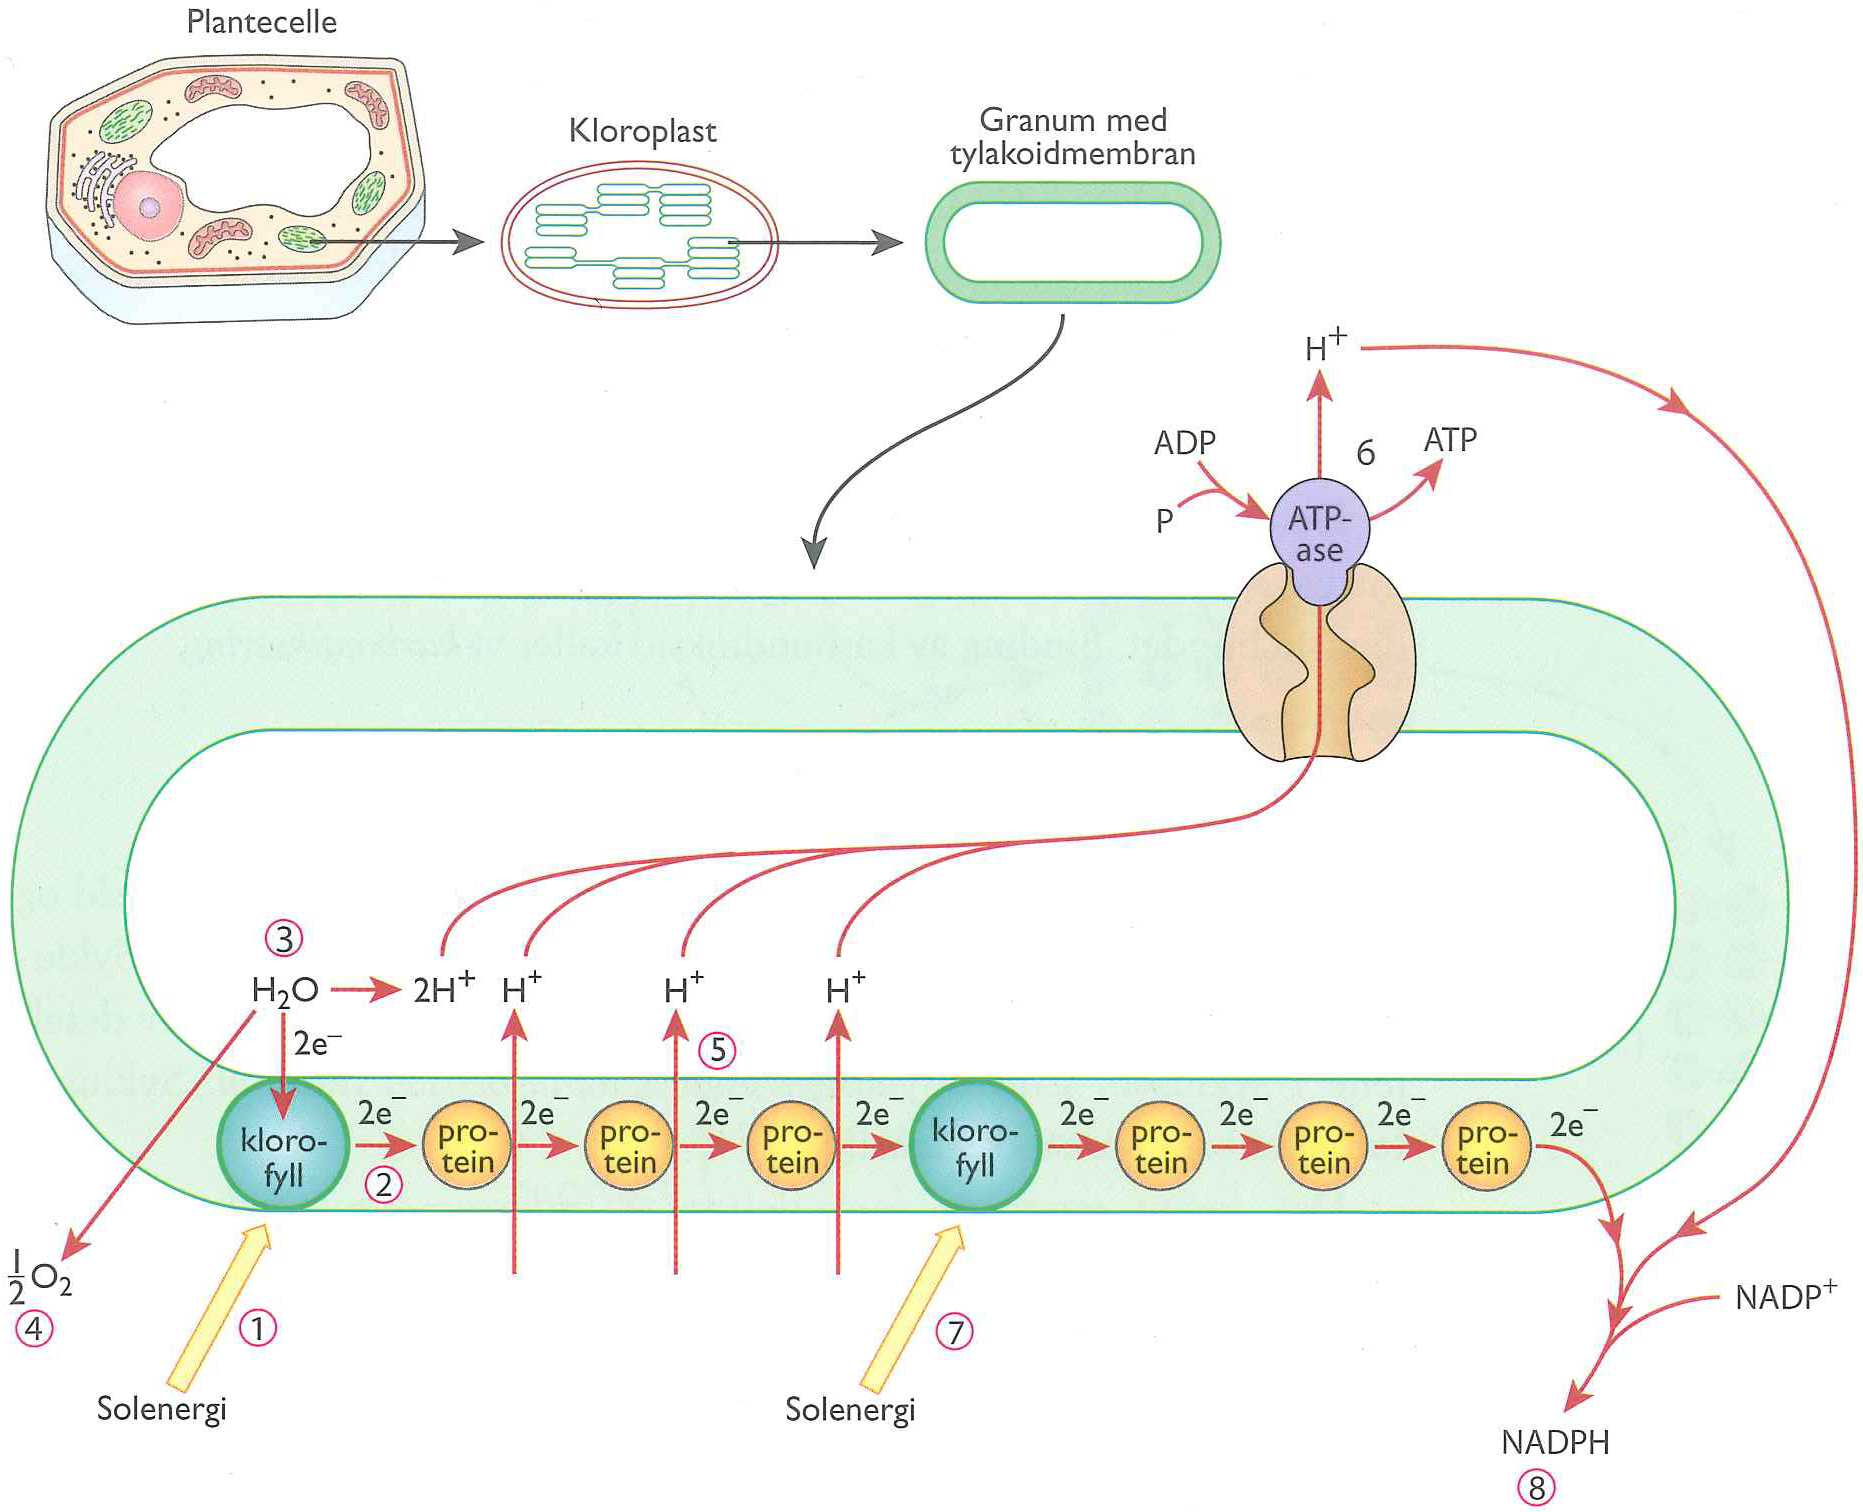
\includegraphics[width=\textwidth]{img/photosynthesis/light_dependent.png}
\caption{Illustration of PS1 and PS2 \citep{bios}}
\label{fig:photosystem}
\end{figure}

\subsection{Light-independent reaction (Calvin-cycle)}
This reaction works as a “sugar-factory”, collecting carbon dioxide and hydrocarbon in many cycles to make glucose. The process takes place in the stroma, and requires the NADPH and ATP generated in the light-dependent reaction \citep{bi2}. 

The glucose produced can be used to generate other organic compounds such as other carbohydrates (ribose, sucrose, starch, glycogen, cellulose), proteins and lipids, depending on what the plant needs.

\subsection{External factors}
Many external factors affect the photosynthesis in plants. As photosynthesis is a relatively inefficient process, using only 8-10\% of the energy in sunlight \citetext{Long et. al, 2006; Zhu et. al, 2010, referenced in \citealp{kirschbaum2011does}}, much research has gone into increasing photosynthesis to achieve greater conversion rates \citetext{Reynolds et al., 2000; Sinclair et al., 2004; Long et al., 2006; Zhu et al., 2010, referenced in \citealp{kirschbaum2011does}}. The factors of significance are \citep{bios}:
\begin{itemize}
\item \ce{CO2} levels
\item Temperature
\item Light intensity and wavelength
\item Water
\end{itemize}
Each of these factors may be a limiting factor, or stressfactor, not enabling photosynthesis to reach its full potential. 

\subsubsection{\ce{CO2} levels}
\ce{CO2} is used in the light-independent reaction for making glucose. The atmosphere contains approximately 0.038\% \ce{CO2}, while the air in e.g. a classroom would most likely contain slightly higher values due to a high concentration of students exhaling \ce{CO2}. In a greenhouse \ce{CO2} levels can get too low, due to a high concentration of plants consuming \ce{CO2} and outputting \ce{O2}. The optimal concentration for most plants is between 0.015\% and 0.05\% \citep{bios}. 


\begin{figure}
        \centering
        \begin{subfigure}[b]{0.45\textwidth}
                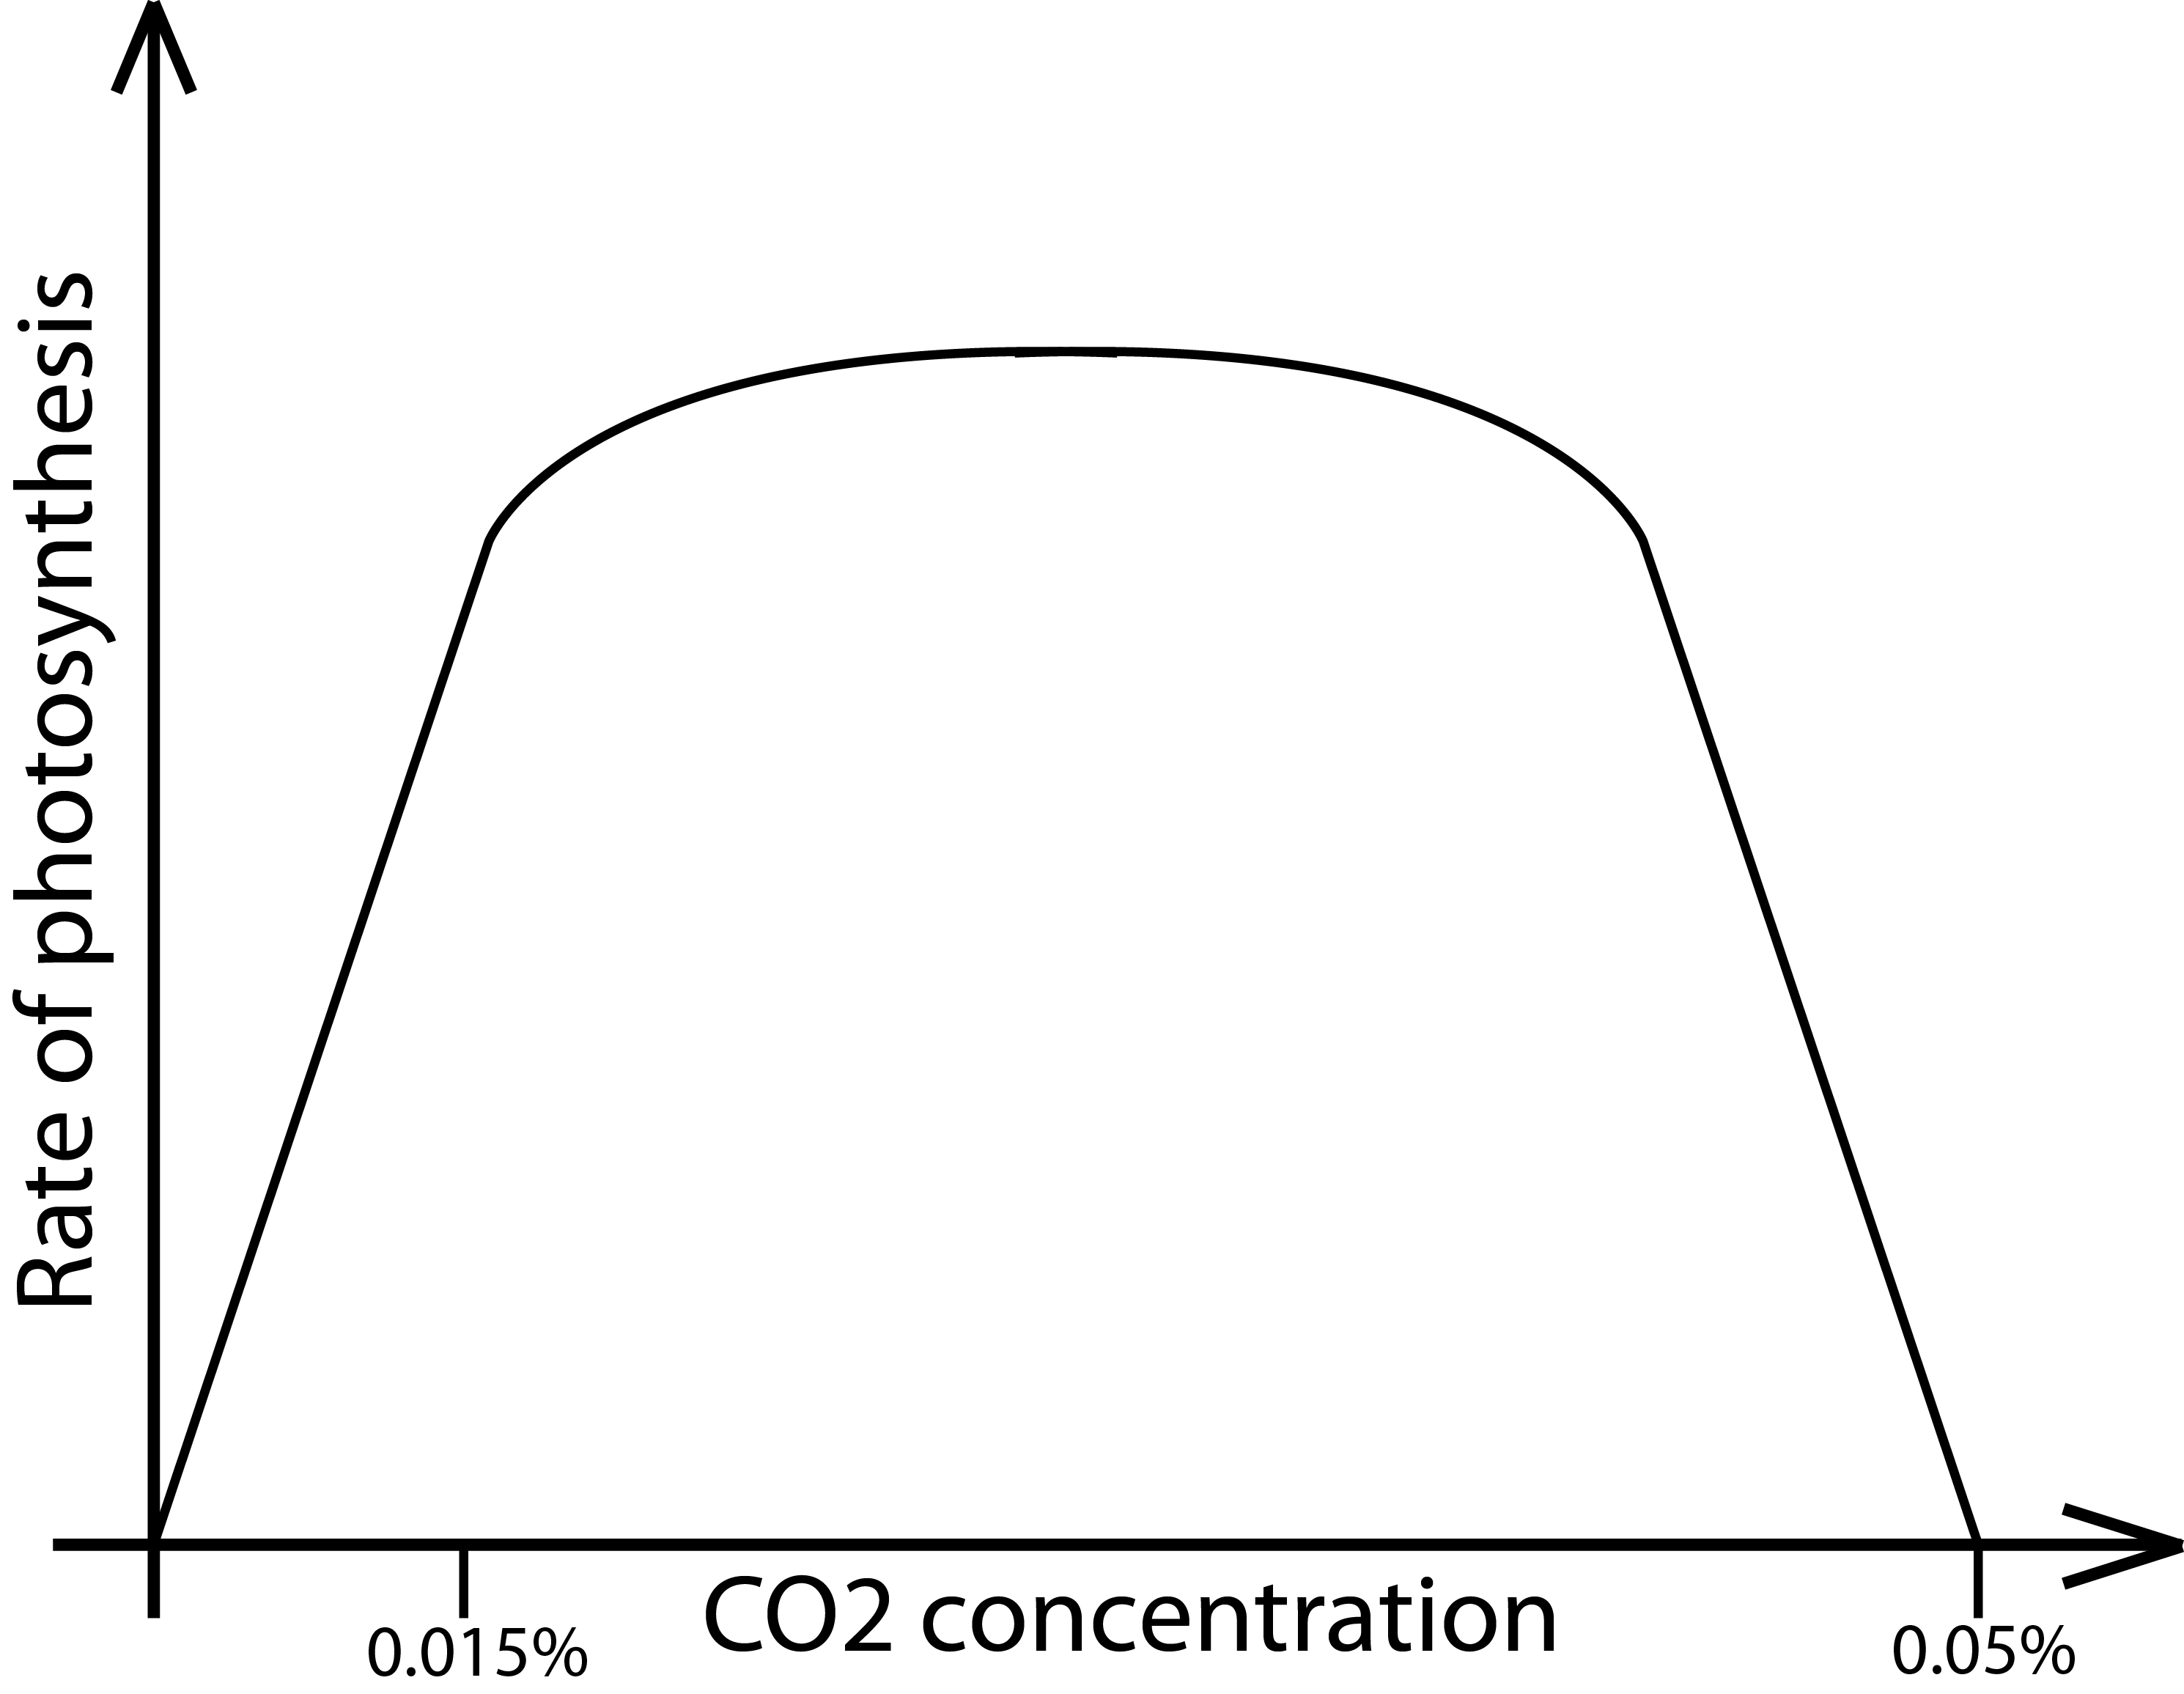
\includegraphics[width=\textwidth]{img/photosynthesis/co2.png}
                \caption{Effect of \ce{CO2} levels on photosynthesis}
                \label{fig:co2levels}
        \end{subfigure}
        ~~
        \begin{subfigure}[b]{0.45\textwidth}
                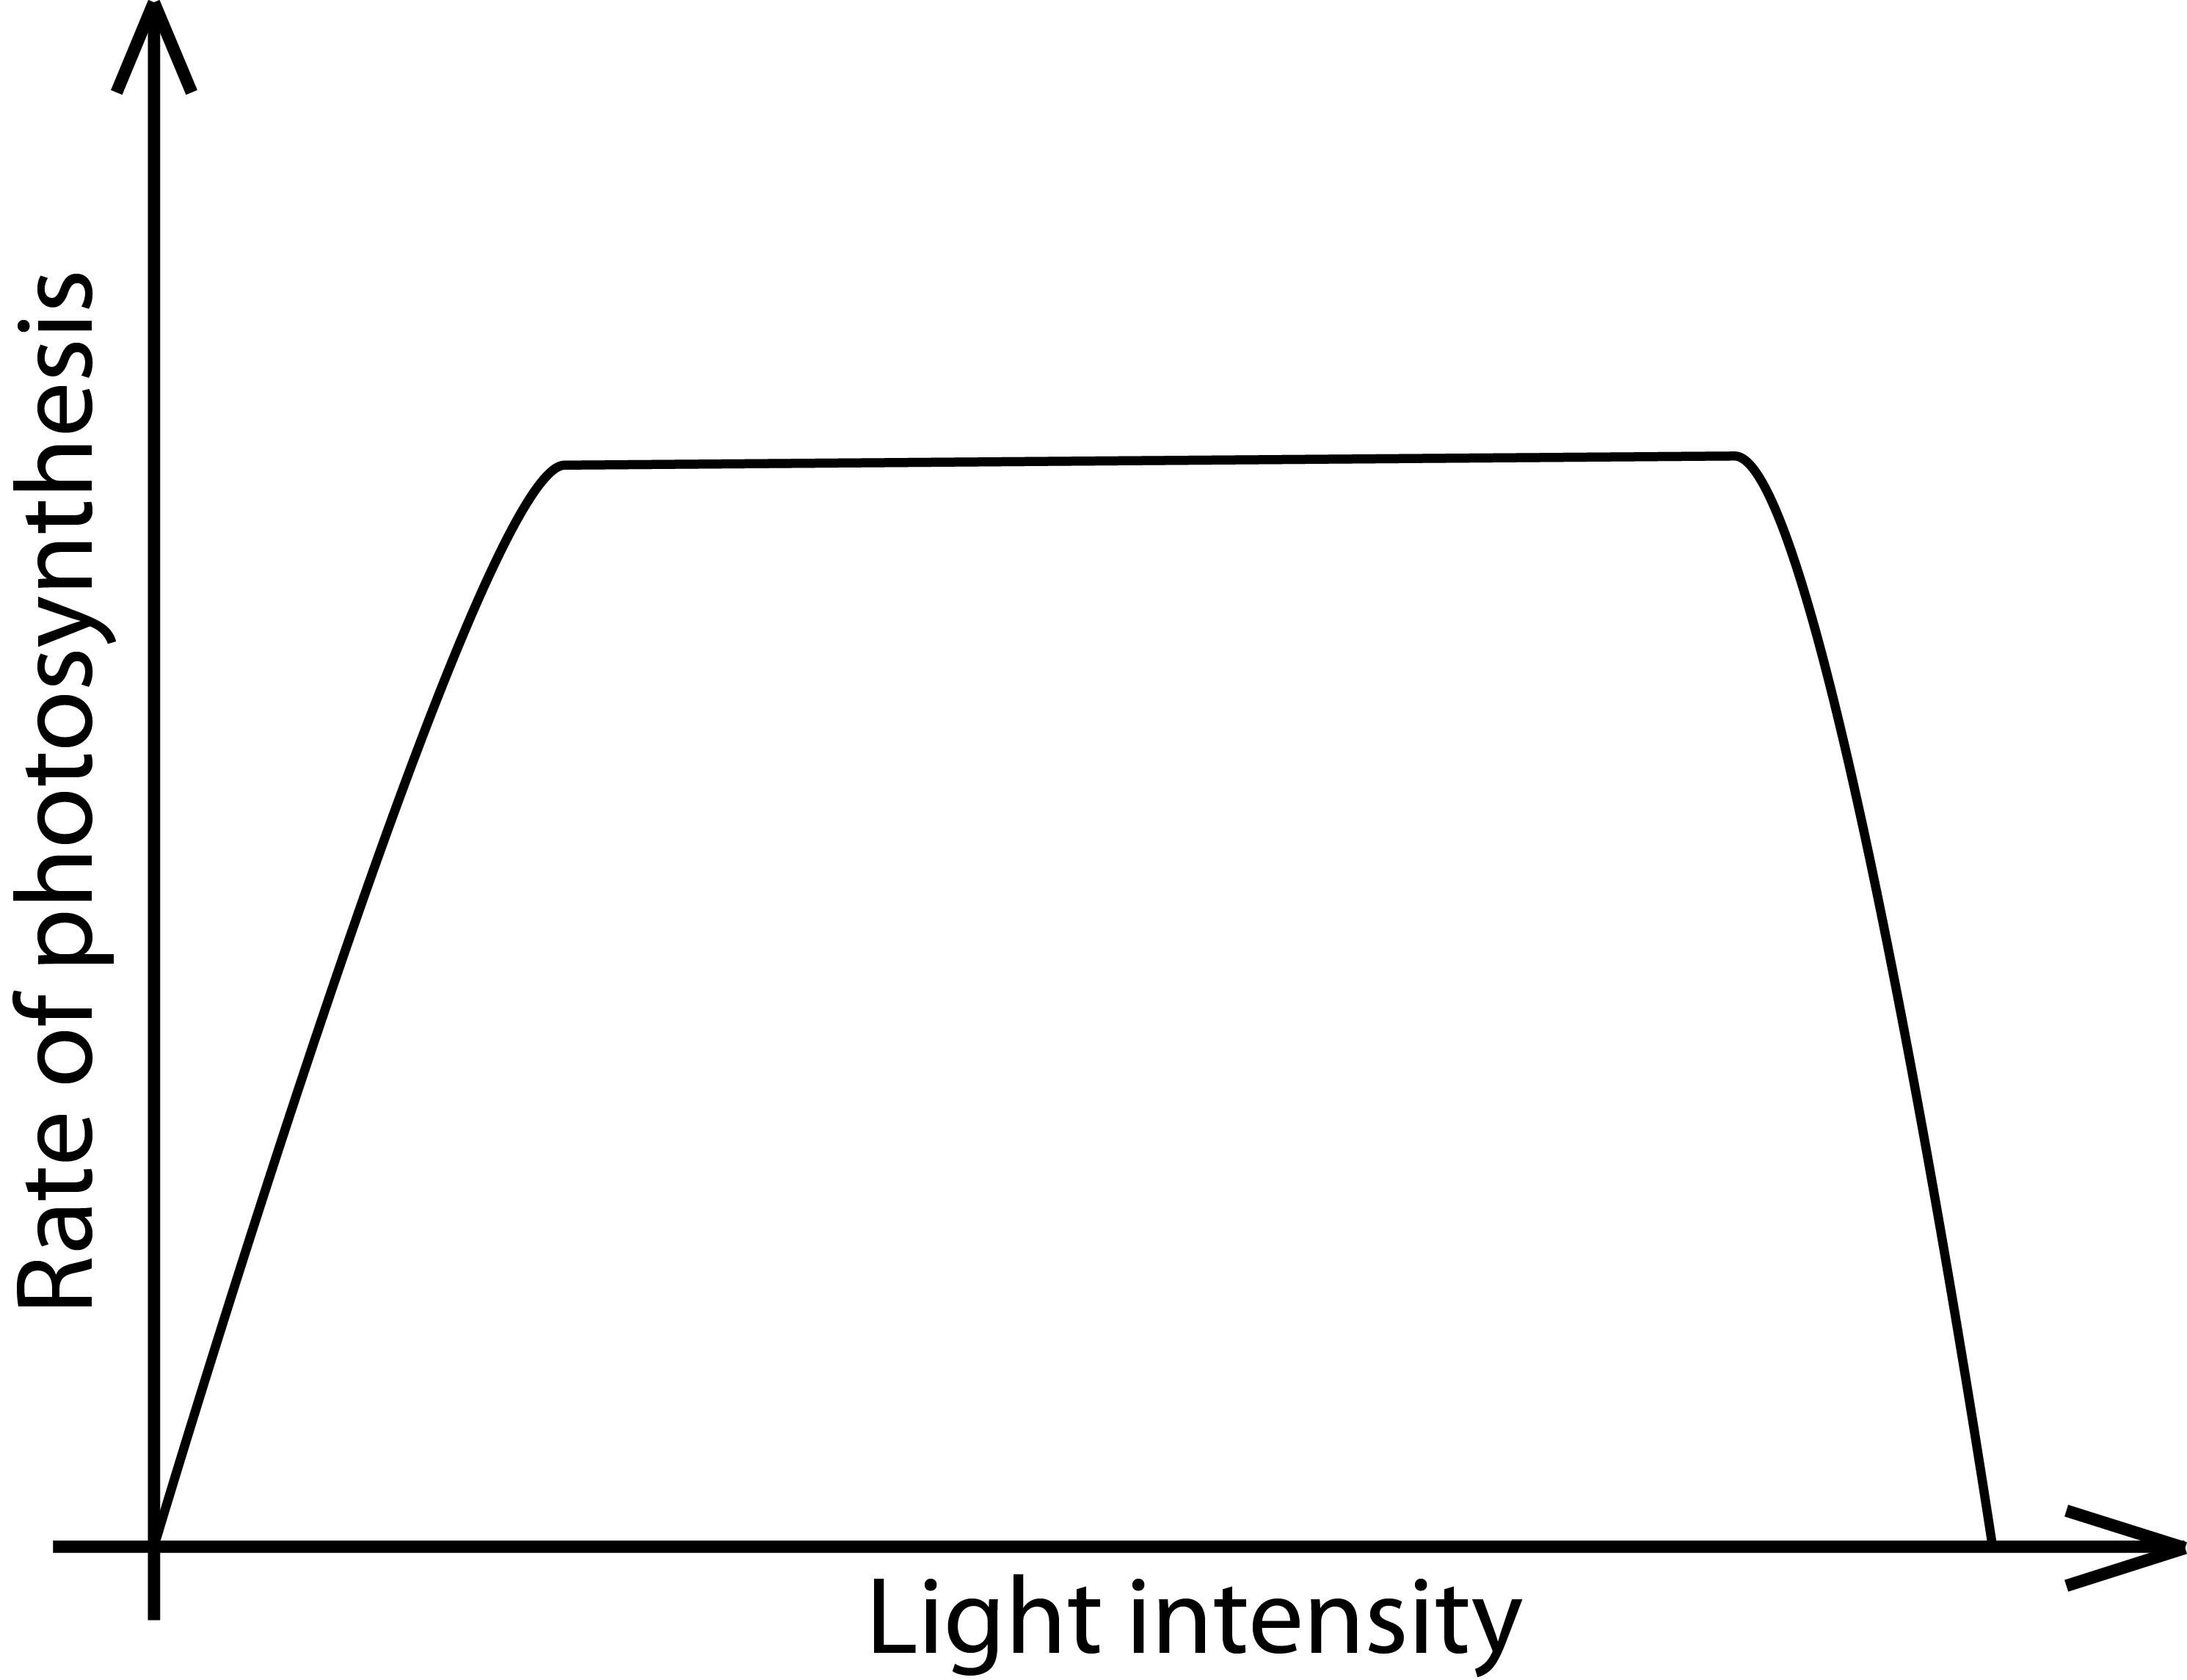
\includegraphics[width=\textwidth]{img/photosynthesis/light_intensity.png}
                \caption{Effect of light intensity on photosynthesis}
                \label{fig:lightintensity}
        \end{subfigure}
       
\end{figure}

\begin{figure}
\centering
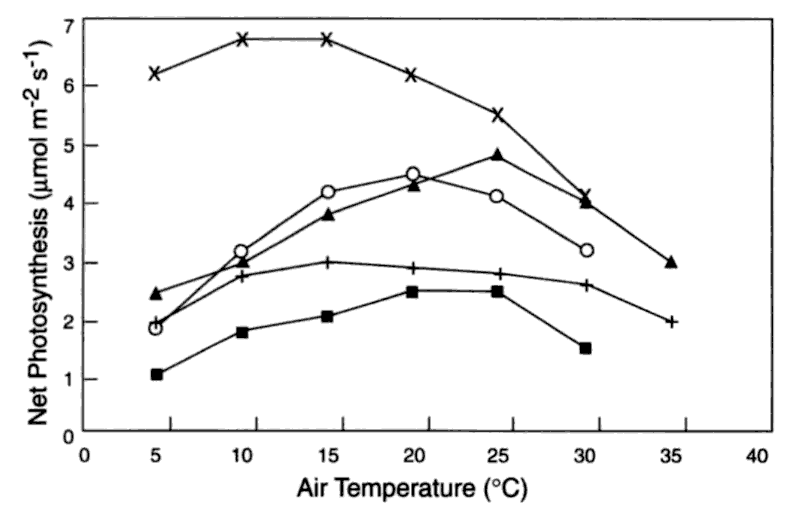
\includegraphics[width=0.75\textwidth]{img/photosynthesis/temperature_new.png}
\caption{Effect of temperature on photosynthesis. Species:
 \textit{\ensuremath{\blacktriangle} Pinus Taeda},  
\textit{\ensuremath{\bigcirc} Pinus Strobus}, 
\textit{\ensuremath{+} Pinus Sylvestris}, 
\textit{\ensuremath{\blacksquare} Picea Engelmanii}, 
\textit{\ensuremath{\times} Pinus Ponderosa}
\citep{hollinger1995external}
}
\label{fig:temperature}
\end{figure}

\subsubsection{Temperature}
All enzymes have an optimal temperature during which they function best \citep{bios}. This temperature may vary from species to species as plants grow in different climates, altitudes and seasons. If the temperature is too low or too high, the molecular structure of the enzymes may be destroyed.

\subsubsection{Light intensity and wavelength}
The different pigments in the light dependent reaction absorb light of wavelengths from (mainly) 400nm to 700nm. Chlorophyll b for instance absorbs blue light (450nm). If a plant with a high concentration of chlorophyll b is not given light of this wavelength, the electrons would not be excited and the reaction in photosystem 2 would not start.

Light intensity also plays a role in this reaction. In low light conditions, there is not enough energy available to excite the chlorophyll molecules, in order to move electrons as needed in PS2. In optimal light conditions, all the chlorophyll molecules are exciting electrons, we say the production is light-saturated. In too strong light conditions, the chloroplasts may burn out from the heat and die.  

\begin{figure}
        \centering
        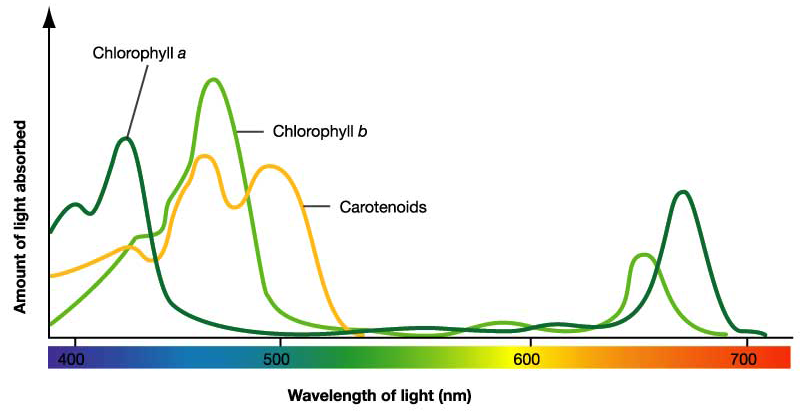
\includegraphics[width=0.8\textwidth]{img/photosynthesis/absorption-spectrum.png}
        \caption{Wavelengths of light absorbed by different pigments}
        \citep{uicbiology}
        \label{fig:wavelengthabsorbtion}
\end{figure}

\subsubsection{Water}
Water is used in both the light-dependent and light-independent reactions, but it is seldom a limiting factor. If water-levels are low and the evaporation-rate is high, most plants will close the leaves to minimize water-loss. This makes the plant unable to absorb \ce{CO2} and photons, which leads to plant reduction \citep{bi2}. Water shortage is only a problem in itself when the plant's cells dries out, leading to the stem and tissue collapsing. 


\section{Koubachi} %Dette er noe dritt! fuck Koubachi. jævla sveitsere
\begin{figure}
        \centering
        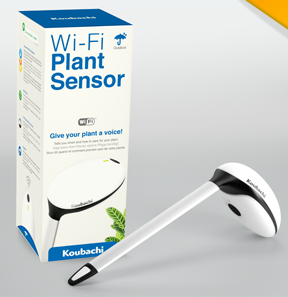
\includegraphics[width=0.4\textwidth]{img/koubachi/sensor.png}
        \caption{Koubachi}
        \label{fig:koubachi}
\end{figure}

Koubachi is a commercial plant monitoring system developed by a company by the same name. The functioning steps of Koubachi is divided in 3: 1.)\emph{Measure}, 2.) \emph{Analyze} and 3.) \emph{Display}. This is done through a sensor unit, the \emph{Koubachi Plant Care Engine (PCE)} and user interfaces in form of a web application and an iOs application \citep{koubachi}. As seen in figure~\ref{fig:koubachidata}, the sensor unit measures soil moisture, temperature and light. The web interface displays the last of the transmitted readings. The koubachi transmits data once every 24 hours in order to save battery life. It does however read data every tenth minute, so the PCE has access to how the environment change over the span of each day.

The PCE is basically an API with the functionality of storing data from sensors, analyzing the data and distributing data and instructions on how and when to care for the plant. Based on plant care models developed by biologists through greenhouse experiments, the PCE can determine the needs of any plant species. Thus, combining the data gathered by the sensor unit with the plant care model, Koubachi provides notifications about how and when to care for your plant. An example of this can be seen in figure~\ref{fig:koubachigraph}, where a graph of light measurements the preceding week i displayed together with a note that \emph{Gretches has too much shade} (Gretches beeing the name of the plant).

\begin{figure}
        \centering
        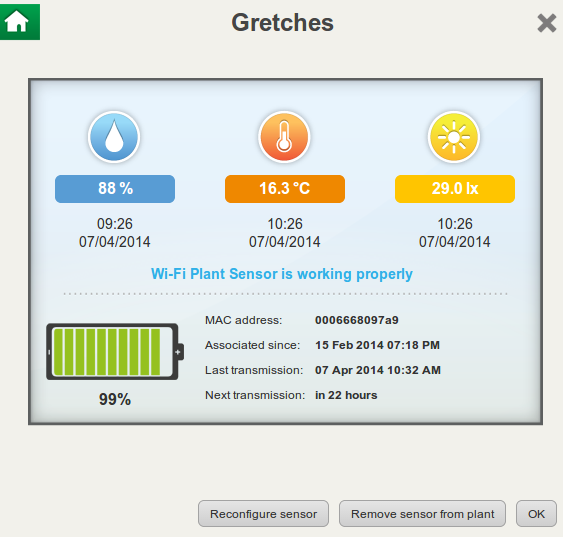
\includegraphics[width=0.8\textwidth]{img/koubachi/instantdata.png}
        \caption{Last data from web interface}
        \label{fig:koubachidata}
\end{figure}

\begin{figure}
        \centering
        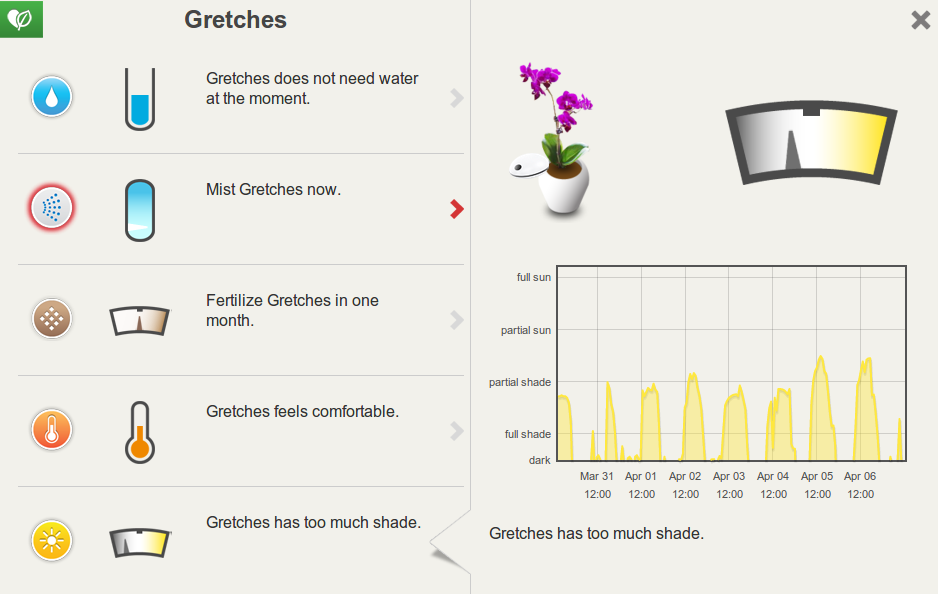
\includegraphics[width=0.8\textwidth]{img/koubachi/lightgraph.png}
        \caption{Light graph from web interface}
        \label{fig:koubachigraph}
\end{figure}

